\chapter{VEGAS Reference}\label{appendix:vegas_reference}

\subsection{VEGAS ADC (MMCM, OGP and INL) Calibration}\label{sec:vegas_adc_calibration}
{\it An understanding of VEGAS ADC calibration is not necessary in order 
to be able to observe with the instrument. It is included here as background 
information only; those who are not interested in it may safely skip to 
section n. The precise method of calibrating the ADCs is still evolving;
this description is correct as of December 2014}

Each VEGAS Bank contains two \glsfirst{ADC} cards, one
for each polarization. The \gls{ADC} cards used are National Semiconductor 
(now Texas Instruments)ADC083000s, which perform 8-bit sampling at 
3 Gigasamples per second (Gs/s). The ADC083000 has a 1:4 demultipexer (data
is output on four busses at a quarter of the \gls{ADC} sampling rate). The outputs
are interleaved to provide output words at the full conversion rate. Use of
these \glspl{ADC} require a number of calibration steps.

\dq{Mixed-mode Clock Management (MMCM)}. The \gls{ADC} clock is driven by the
\gls{FPGA} on the Roach II card.The \dq{MMCM phase calibration}, consists of
calibrating the \gls{FPGA} clock phase relative to the \gls{ADC} inputs to
avoid glitches when the  \gls{FPGA} captures the data samples. The MMCM
calibration depends on the mode (\gls{FPGA} clock frequency and BOF file) in use.

MMCM calibration is performed automatically by the VEGAS Manager, whenever
a new mode is selected. This calibration step is stable and routine.

\dq{Offset, Gain and Phase (OGP)}. Each core of the \gls{ADC} may have a
separate Offset, Gain and Phase. Currently, these are calibrated off-line, by
injecting a test-tone, and adjusting the offset, gain and phase of the
\gls{ADC} counts to match the injected tone as closely as possible. 
Once the OGP calibration has been performed, the optimum values
are stored in the VEGAS config file, and downloaded by the Manager to the
firmware whenever the mode changes.  The OGP values also depend on the mode 
(the \gls{FPGA} clock frequency) in use. 

\dq{Integral non-linearity (INL)}. INL is a measure of the deviation of
each individual 8-bit value from a straight line through the input to
output transfer function. The deviation of any given value from a straight
line is measured from the center of that value. INL calibration is also
done off-line. It is independent of VEGAS Mode, so the appropriate values
are stored in the config file, and simply downloaded to the hardware when
the manager is turned \dq{ON}.


\subsection{IF Levels and Balancing}\label{sec:vegas_balancing}

Once the \gls{IFsys} system from the receiver to the IF rack is balaned, 
the VEGAS balance \gls{API} then adjusts the attenuators in the converter rack
to balance the power level at the inputs to the VEGAS \glspl{ADC} to be
(by default) -20dBm.

For VEGAS modes higher than three, digital filters are implemented in the
\gls{FPGA}. The filtered output is requantized to 8 bits; a digital gain
adjustment is implemented in the \gls{FPGA} to scale the digital filter
output values so that there will be no overflow after requantization. 

Both of these steps are performed when the \gls{Astrid}
{\bfseries{\textcolor{pythonKeywords}{Balance}}()} directive is
issued. A new keyword has been added to the
{\bfseries{\textcolor{pythonKeywords}{Balance}}()} python dictionary 
(see Appendix~\ref{appendix:advutil}) which can be used to change the
target input level to VEGAS, for example:

{\tt Balance('VEGAS', {'target\_level':-20})}

will set the input target level to -20 dBm for both the \gls{ADC} and requantizer
balannce.

The \gls{IF} system must be able to handle the large bandwidths all
the way to VEGAS, which then splits the signal into the more narrow 1.25 GHz
bandwidths of the individual VEGAS banks. This can be problematic, as part
of balancing the  entire bandwidth is based on the signal received by a single
VEGAS bank. After the correct attenuation is set at the converter module for
one bank, the system can potentially require amplification for other portions
of the bandpass. This can cause the system gain to transition to the non-linear
regime, where changes in the input signal do not linearly change the recorded output. 
We have found that using when using a 3.5 GHz bandwidth, the system was able 
to properly configure across all frequencies. We were not able to sufficiently 
test using larger than 3.5 GHz of total observed bandwidth across the system. 
It is recommended that users hoping to push the bandwidth limit should watch 
the attenuation levels in the converter module, and if necessary discuss the
optimum settings with their support scientist.


\subsubsection{vegas\_status}\label{sec:vegas_status}
{\it This section is only relevant for advanced diagnosis of VEGAS problems.
It may be skipped by the average Observer.}

VEGAS utilitizes eight high performance computers (HPCs), one for each Bank.
Each HPC contains a Graphics Processor Unit (GPU) which is used to perform
much of the digital processing for modes 4 and above. These HPCs are also
responsible for collating metadata, and writing this plus the actual spectra to
disk. These machines are called {\tt VEGAS-HPC1} through {\tt VEGAS-HPC8}.

VEGAS meta-data is stored in shared memory on these machines, and it is 
possible to monitor the status of this meta-data as follows:

\begin{verbatim}
ssh into the machine of interest, then
% source /home/gbt/gbt.bash (or .csh)
% vegas_status
\end{verbatim}

This will bring up a terminal status display, as shown in 
Figure~\ref{fig:vegas_status}.

Observer's should not normally need to use this tool, but it is possible on
occasion that by running it they might be able to give support scientists /
engineers some useful information in the case of problems.

\begin{figure}[!h]
\begin{center}
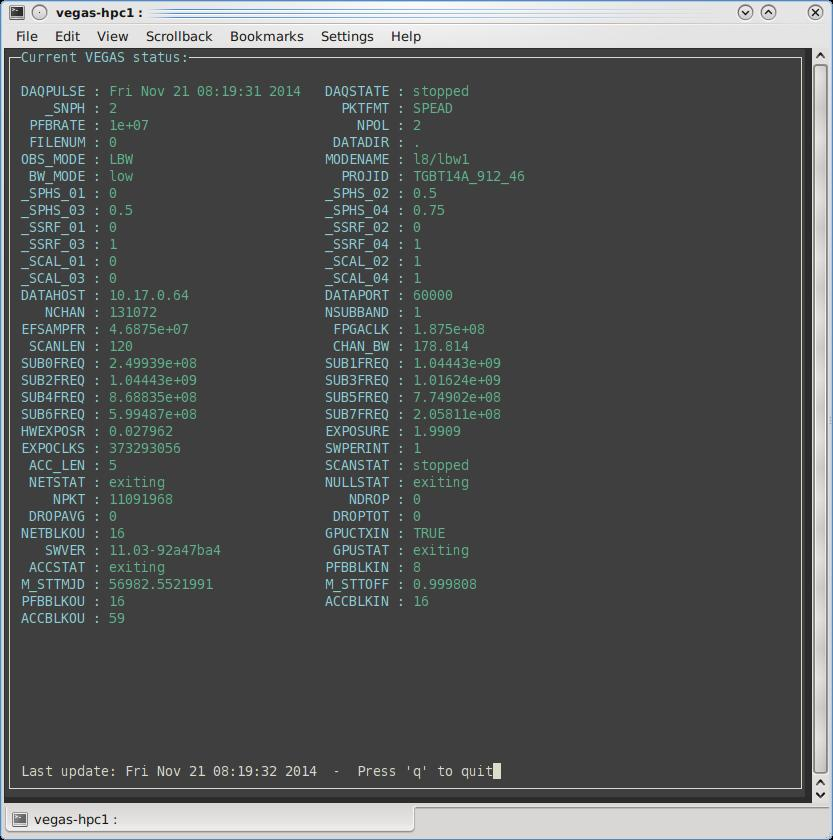
\includegraphics[width=5.5in]{vegassharedmemory.jpg}
\caption[The VEGAS shared memory screen]{The VEGAS shared memory screen}
\label{fig:vegas_status} 
\end{center}
\end{figure}

\section{Baseline Performance}\label{sec:vegas_baselines}

Gain variations across the large bandpasses desired in radio astronomy 
require significant efforts to balance and stabilize. These variations 
create baselines that are not perfectly flat and can potentially vary with 
time. Thorough data calibration helps to mitigate these effects, but 
calibration can only be effective if the baselines are stable. 
With this in mind, developing the VEGAS infrastructure has focused on the 
temporal and spectral stability of baselines. It has served as an 
interesting engineering problem to create an IF system that is capable and 
stable for all receivers. In this section, we will discuss the status of 
the baselines as recorded by VEGAS.

The baseline shapes come from two main causes; variations due to the 
receiver and IF system, and shapes due to digital filters within VEGAS. 
Figure~\ref{basicbaselines} shows the baselines types expected from VEGAS. 
While not flat, all of these baseline shapes have been found to be stable 
out to at least 30 minutes, and are easily removed with standard 
calibration techniques

\begin{figure}
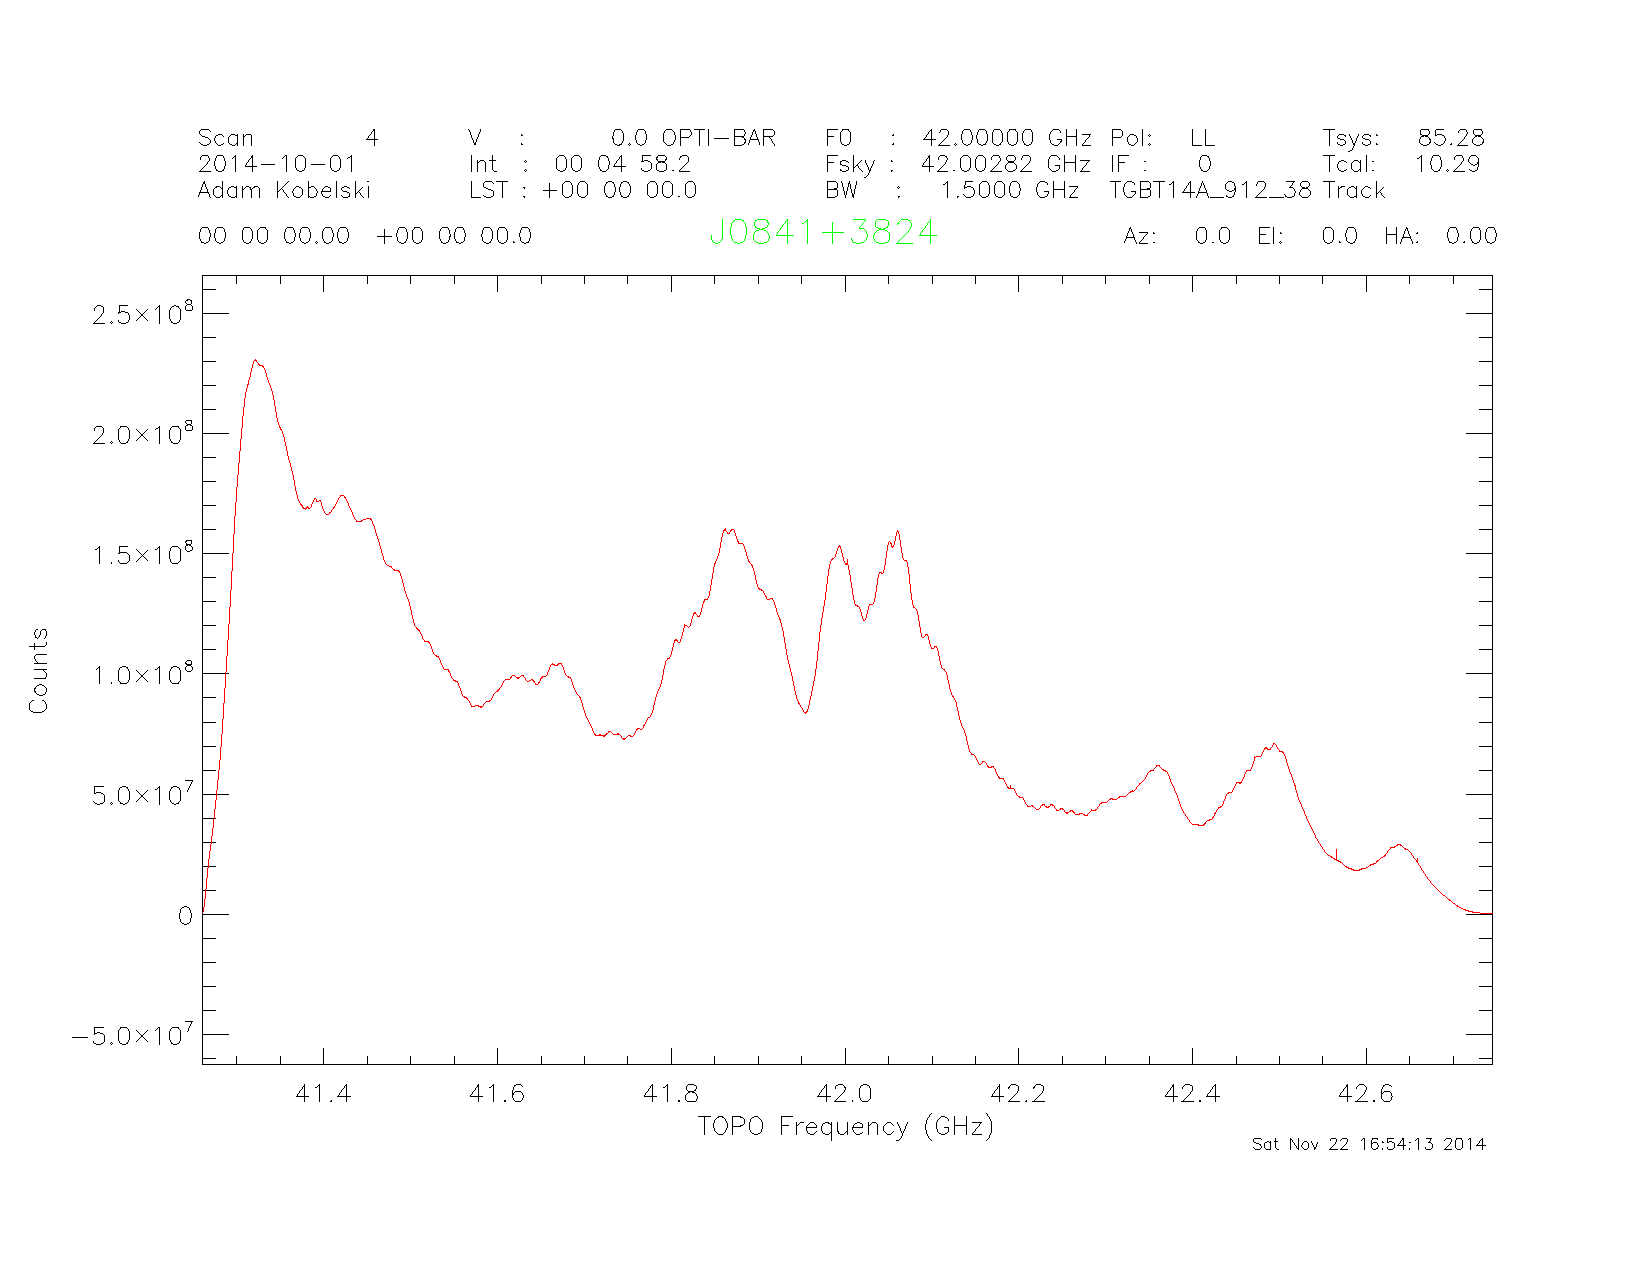
\includegraphics[width=0.5\linewidth]{mode2bandpass.pdf}
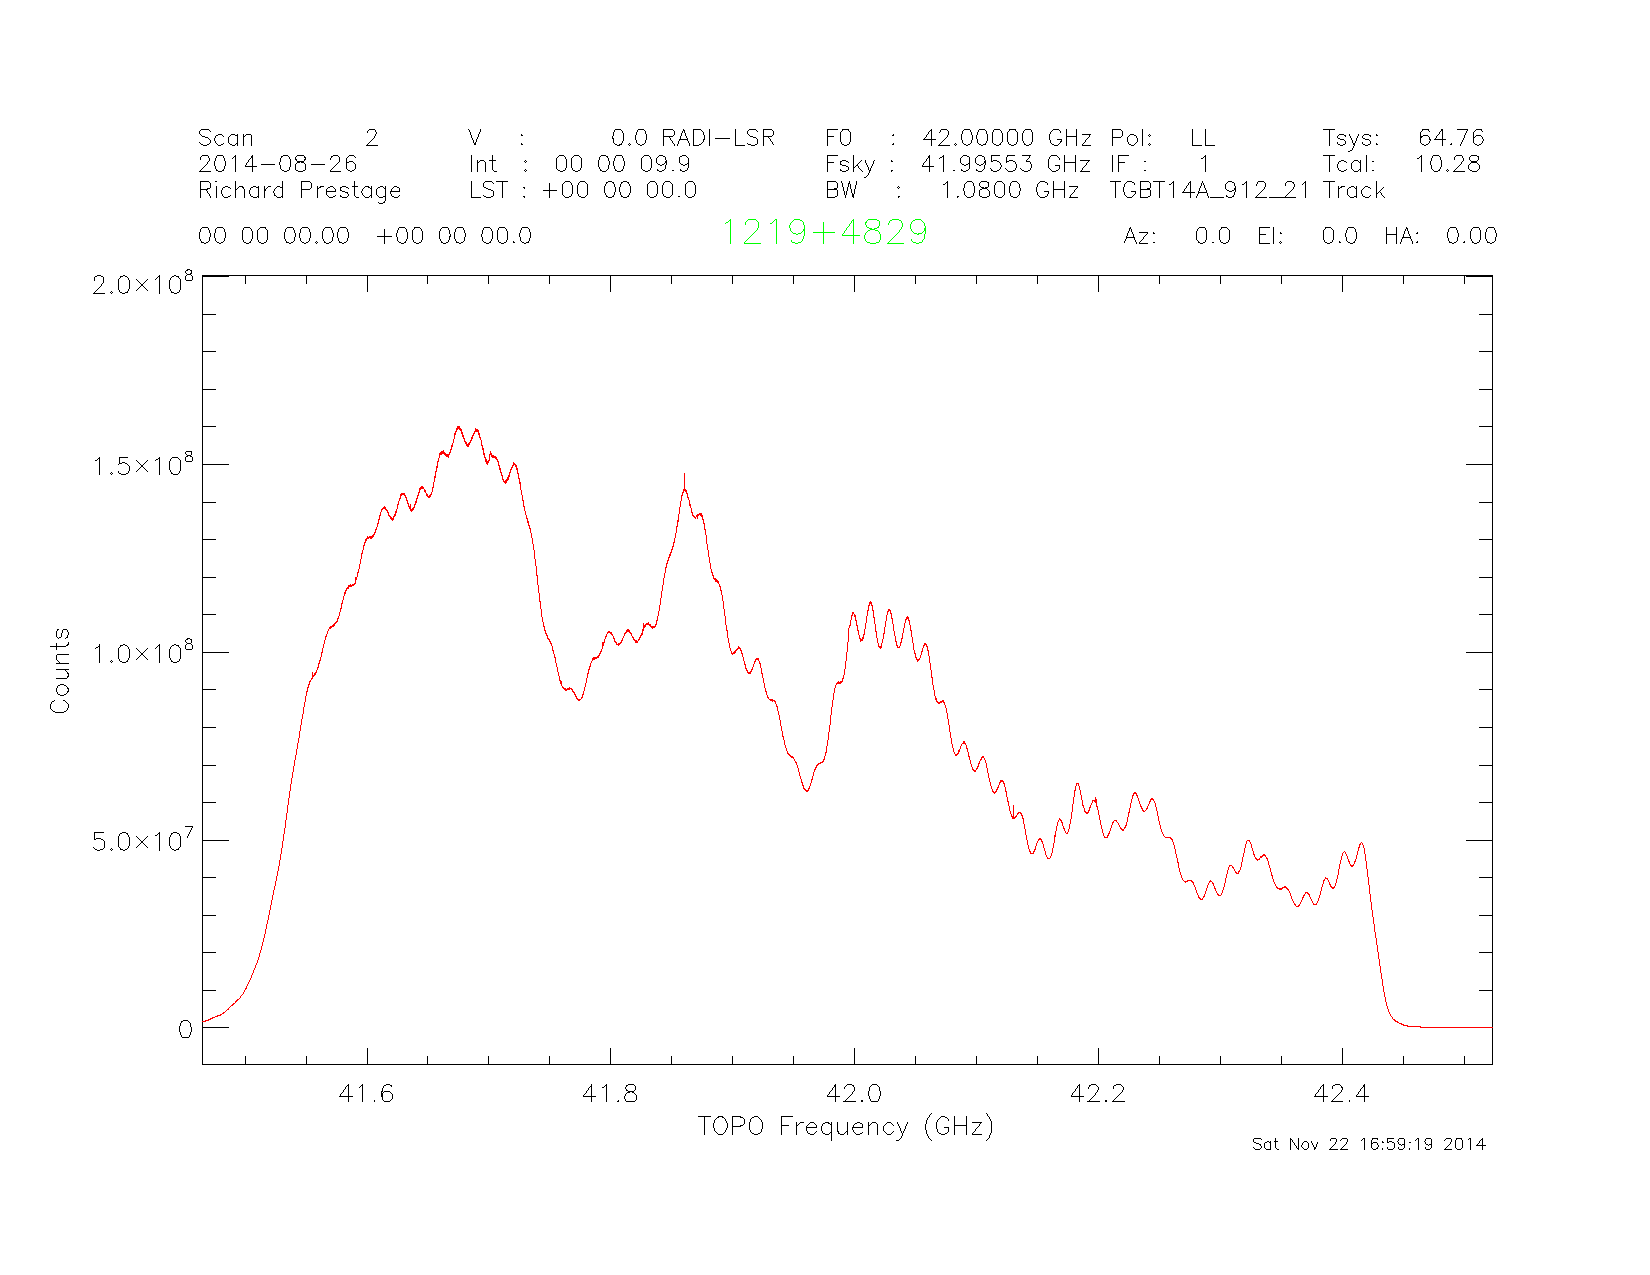
\includegraphics[width=0.5\linewidth]{mode3bandpass.pdf}
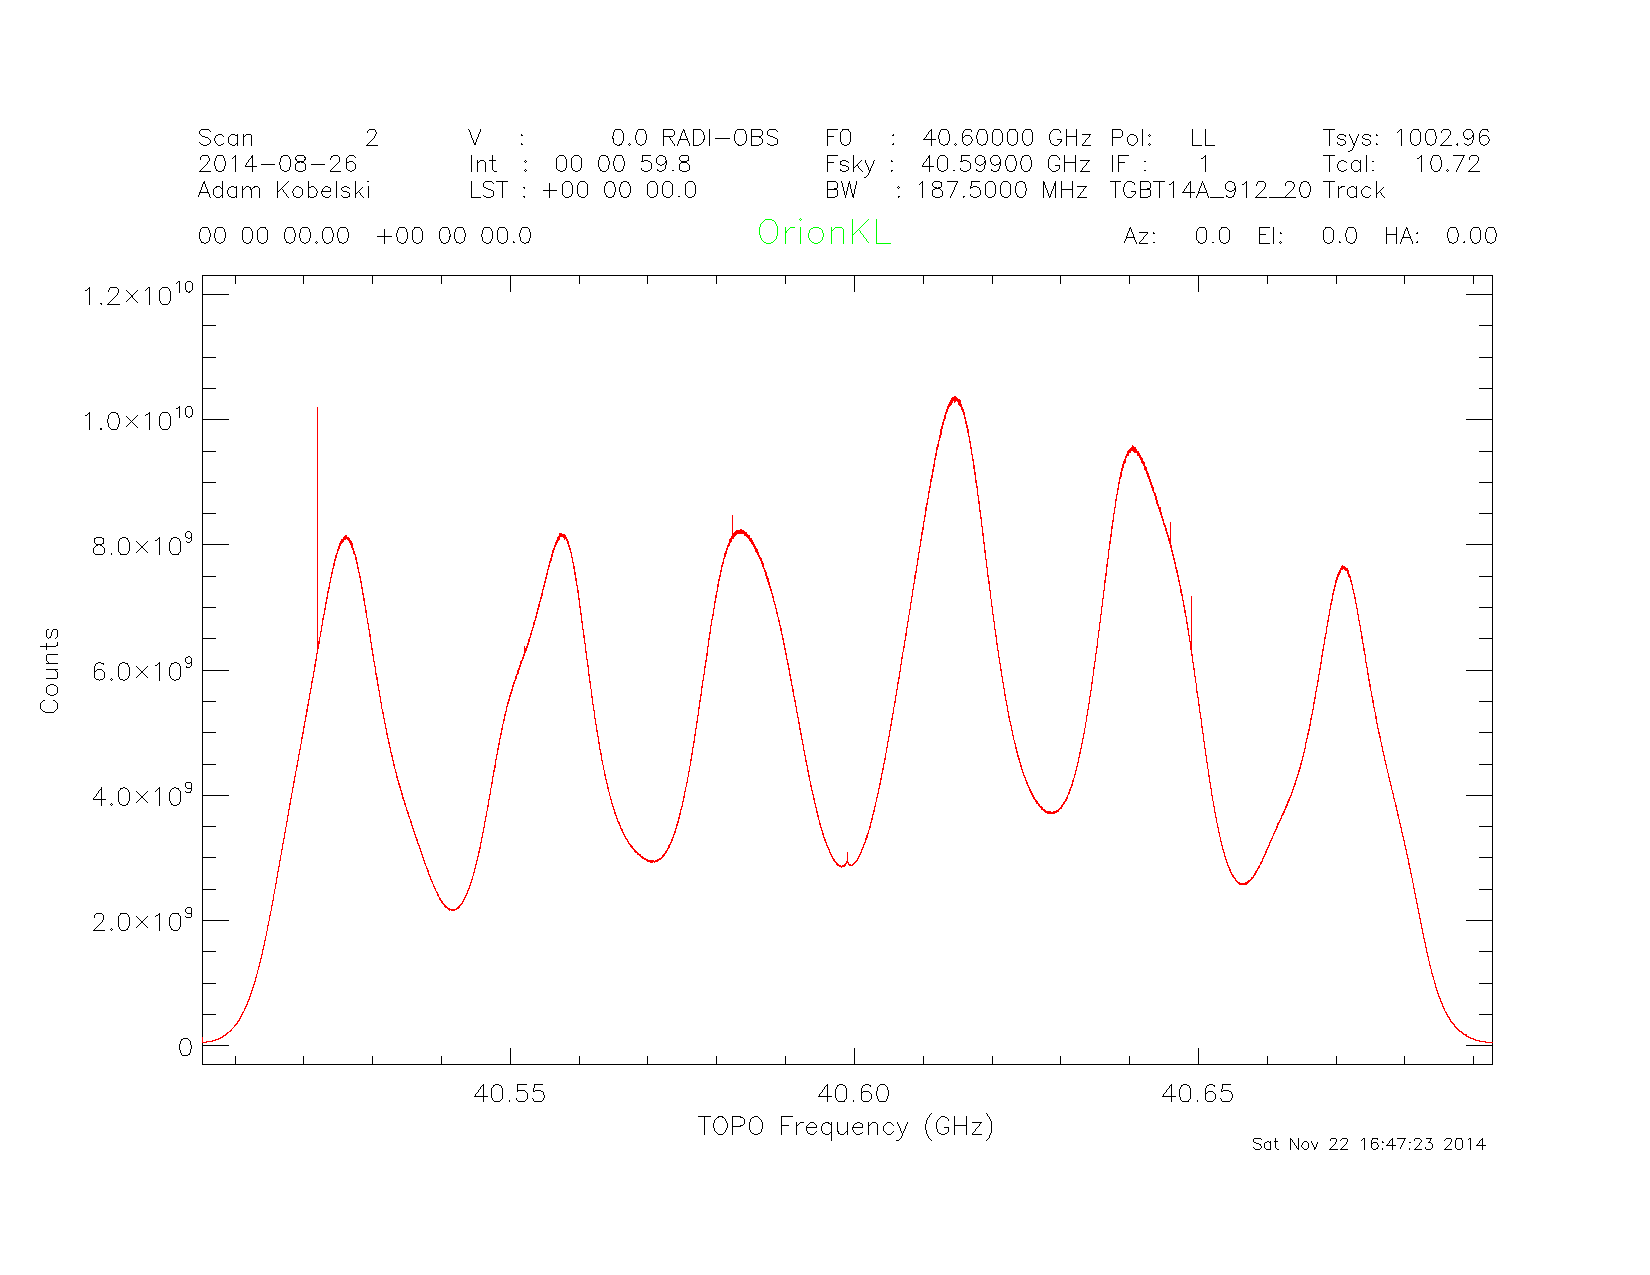
\includegraphics[width=0.5\linewidth]{mode4bandpass.pdf}
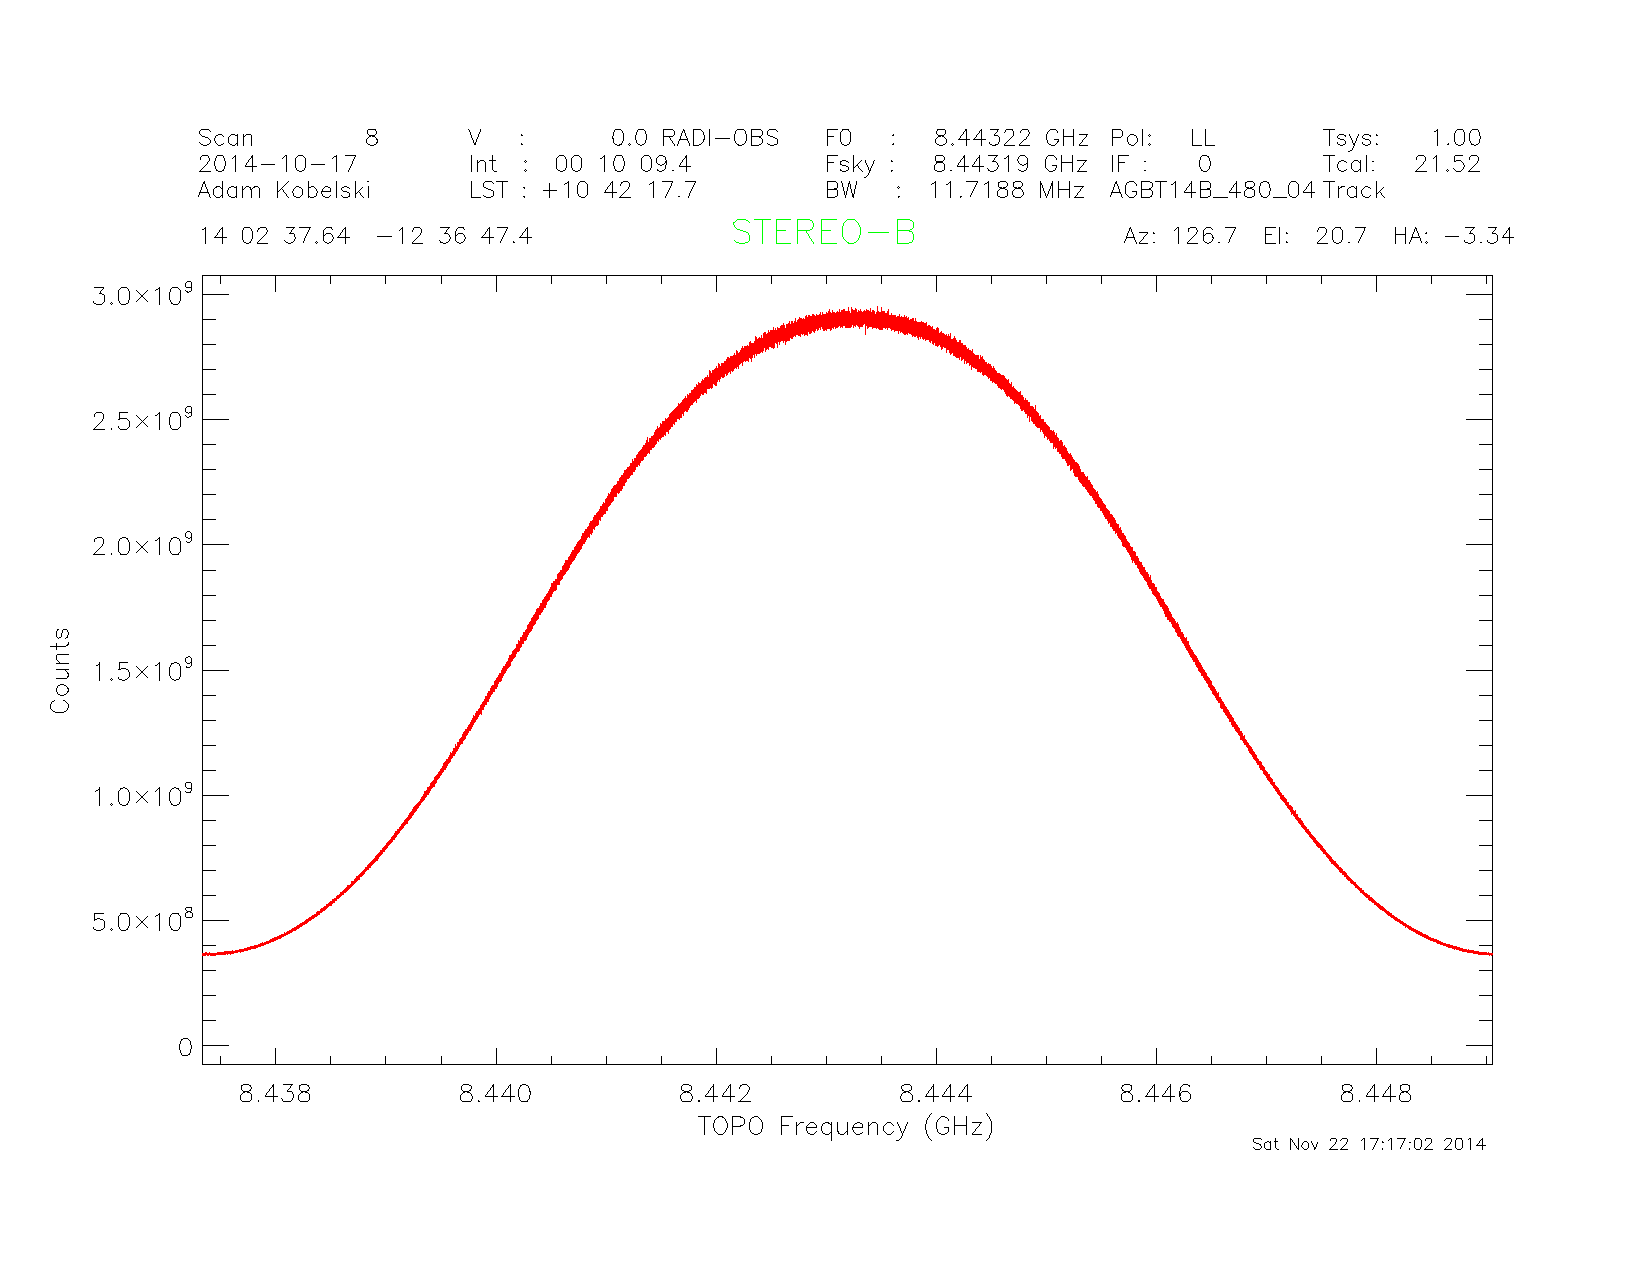
\includegraphics[width=0.5\linewidth]{mode17bandpass.pdf}
\caption[VEGAS bandpass for the four families of VEGAS modes]
{VEGAS bandpass for the four families of VEGAS modes. The upper 
left represents the 1500 MHz bandwidth of modes 1 and 2, the upper right is 
mode 3, the lower left shows the bandpass for mode 4 (modes 4-9 all show a 
similar bandpass), mode 17 (representing modes 10-29) is shown in the 
lower right. These shapes are all extremely stable, and so are readily 
removed by the standard calibration schemes. Note the high frequency 
ripples shown in the mode 3 plot were caused by a standing wave in the 
cable between the IF Rack and VEGAS; attenuators have been added to the cable
 to remove this ripple (hence it is not seen in the mode 2 data taken later).\label{basicbaselines}} 

\end{figure}

When looking at Figure~\ref{basicbaselines}, the ripples in the mode 4-9 data 
(lower left) stand out. This pattern is caused by the Finite Impulse Response
(FIR) filter used in the digital processing of low bandwidth modes. This 
pattern is stable, and as long as the amplification within the IF system is 
kept in the linear regime (see Section~\ref{sec:vegas_balancing}), 
this pattern will not effect the final calibrated data. Modes 10-29 show 
a similar pattern, with just a single ripple.

Secondary ripples (10MHz wide) are visible in the mode 3 bandpass shown in 
the upper right of Figure~\ref{basicbaselines}. These ripples are due to a 
standing wave in the cabling between the Converter Rack and VEGAS. 
Placing attenuation on the cables at the converter rack minimizes these 
standing waves while leaving the signal strength and 
signal-to-noise ratio of the signal intact. The ripples in the mode 2 
image (upper left) have a lower amplitude, since this data was taken with the 
attenuation in place.

{\bf In the next version of this guide, we will replace the mode 3 figure 
with one taken after the attenuators were in place.}

As mentioned previously, the stability of the baseline is more important 
than the overall baseline shape. The thermal stability 
of the system greatly impacts the temporal stability of the baselines. 
We have attempted to isolate all cables and VEGAS itself to minimize 
these impacts, and are currently in the process of further improving the 
thermal isolation of the system. The calibration of the digital systems 
within VEGAS can also affect the temporal stability of the baselines; 
the software/digital team has worked diligently to successfully track down 
and alleviate these issues.

Removal of all baseline shapes is not feasible, so it is important to 
account for these shapes in data calibration. This is most often 
accomplished by using position switching (obtaining data when pointing on 
and off source) and/or frequency switching (shifting the central frequency 
such that the desired spectral lines appear at different locations 
within the bandpass shape). If the shape of the baseline is still of concern 
after these types of calibration, it is recommended to look into 
vectorized baseline removal (such as described in  Winkel, Kraus, 
\& Bach (2012) \url{http://adsabs.harvard.edu/abs/2012A%26A...540A.140W}).

\section{VEGAS and Deep Integrations}\label{sec:vegas_deep_integrations}

At the time of writing (December 2014), we have not extensively tested the
performance of VEGAS for deep integrations.

However, some science observations have been performed with VEGAS at Q-band,
looking for high-redshifted CO lines. Figure~\ref{fig:vegas_deep_integrations}
shows the result of four and a half hours of effective integration time
using the ``sub beam nod'' observing technique (D. Frayer, private
communication). The previous vector calibration, as applied for example to
the GBT spectrometer yields bad baselines with VEGAS. However, a simple
scalar $T_{sys}$ calibration works well, when applying an appropriate high-pass
filter to remove large-scale smooth frequency structures. The sub beam nod
observations were taken with a nod period of 6 seconds, and 0.2 second 
integration times to minimize the blanking. The high frequency ripples then
present in VEGAS data, and the ``spikes'' (see \S~\ref{sec:vegas_spike}
calibrate away nicely. This spectrum consists of 4 overlapping Mode 1 
spectra; no special processing was required to ``stich'' the spectra
together; overlapping channels were simply dropped. After the above processing
was performed, the scalar processing yielded a nice flat baseline, and
noise that is consistent with the radiometer equation.

\begin{figure}[!h]
\begin{center}
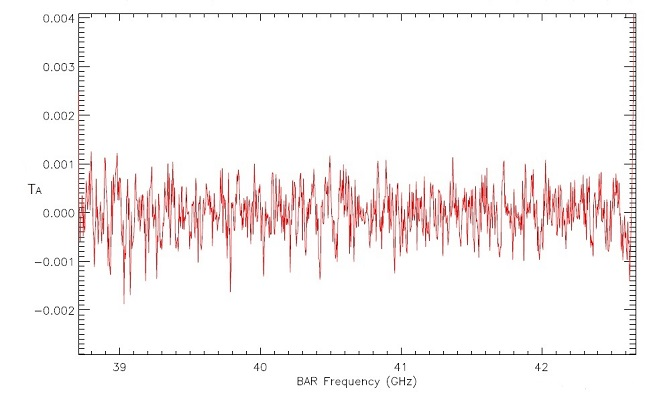
\includegraphics[width=5.5in]{deepIntegration.jpg}
\caption[A deep integration with VEGAS]{A deep integration with VEGAS\label{fig:vegas_deep_integrations}} 
\end{center}
\end{figure}


\section{The Spurs}\label{sec:vegas_spurs_detailed}
When attempting to search for \gls{RFI} with VEGAS by running a high-pass
filter through the data, significantly more spikes/spurs were found than
naively expected. These spurs could be found in the same bins in relatively
RFI free wavelengths, such as \gls{Qband}. The spurs appear at the same
location (in bin space) for a given mode and have relatively stable
amplitudes. These faint spurs are not always directly visible in the data,
but became clear when high-pass filtered, as shown in
Figure~\ref{fig:vegas_spurs}. After significant testing, it was determined
that these spurs are below the spurious-free dynamic range of -60dBc
specified by the manufacturer, and cannot be fully removed.
In overly simplistic terms, the spurs are caused by the leaking of the 
\gls{FPGA} clock into the four interleaved \glspl{ADC}.

In overly simplistic terms, the spurs are caused by the leaking of the 
FPGA clock into the four interleaved ADCs. This causes a rail of thin 
spikes/spurs to be inserted into the VEGAS IF spectrum at frequencies:
\begin{equation}
\nu_{\rm spurs}=\frac{i*f_{\rm  s}}{64},
\end{equation}

\noindent where 0$\le i \le$64 and $f_{\rm s}$ is the sample rate of the ADC. 
Since the bandwidth of the FFT can only be half of $f_{\rm s}$, $i$ actually 
runs from 0$\le i \le$32, meaning there will never be more than 33 spurs in 
a given data set\footnote{The 33$\le i \le$ 64 spurs alias back to the 
0$\le i \le$ 32 spurs when creating the power spectrum}. 
Note that these frequencies are relative to the intermediate frequency input 
into VEGAS, so they should be offset by $\nu_{\rm V,c}$ (the centered VEGAS 
specific intermediate frequency) and $\nu_{\rm s,c}$, the center sky 
frequency, such that the spurs will occur at sky frequencies

\begin{equation}\label{eq:vegas_spikeeq}
\nu_{\rm spurs,sky}=\nu_{\rm s,c}+(\nu_{\rm spurs}-\nu_{\rm V,c}),
\end{equation}

\noindent as shown in Figure~\ref{fig:vegas_spurcalc}.

\begin{figure}[h]
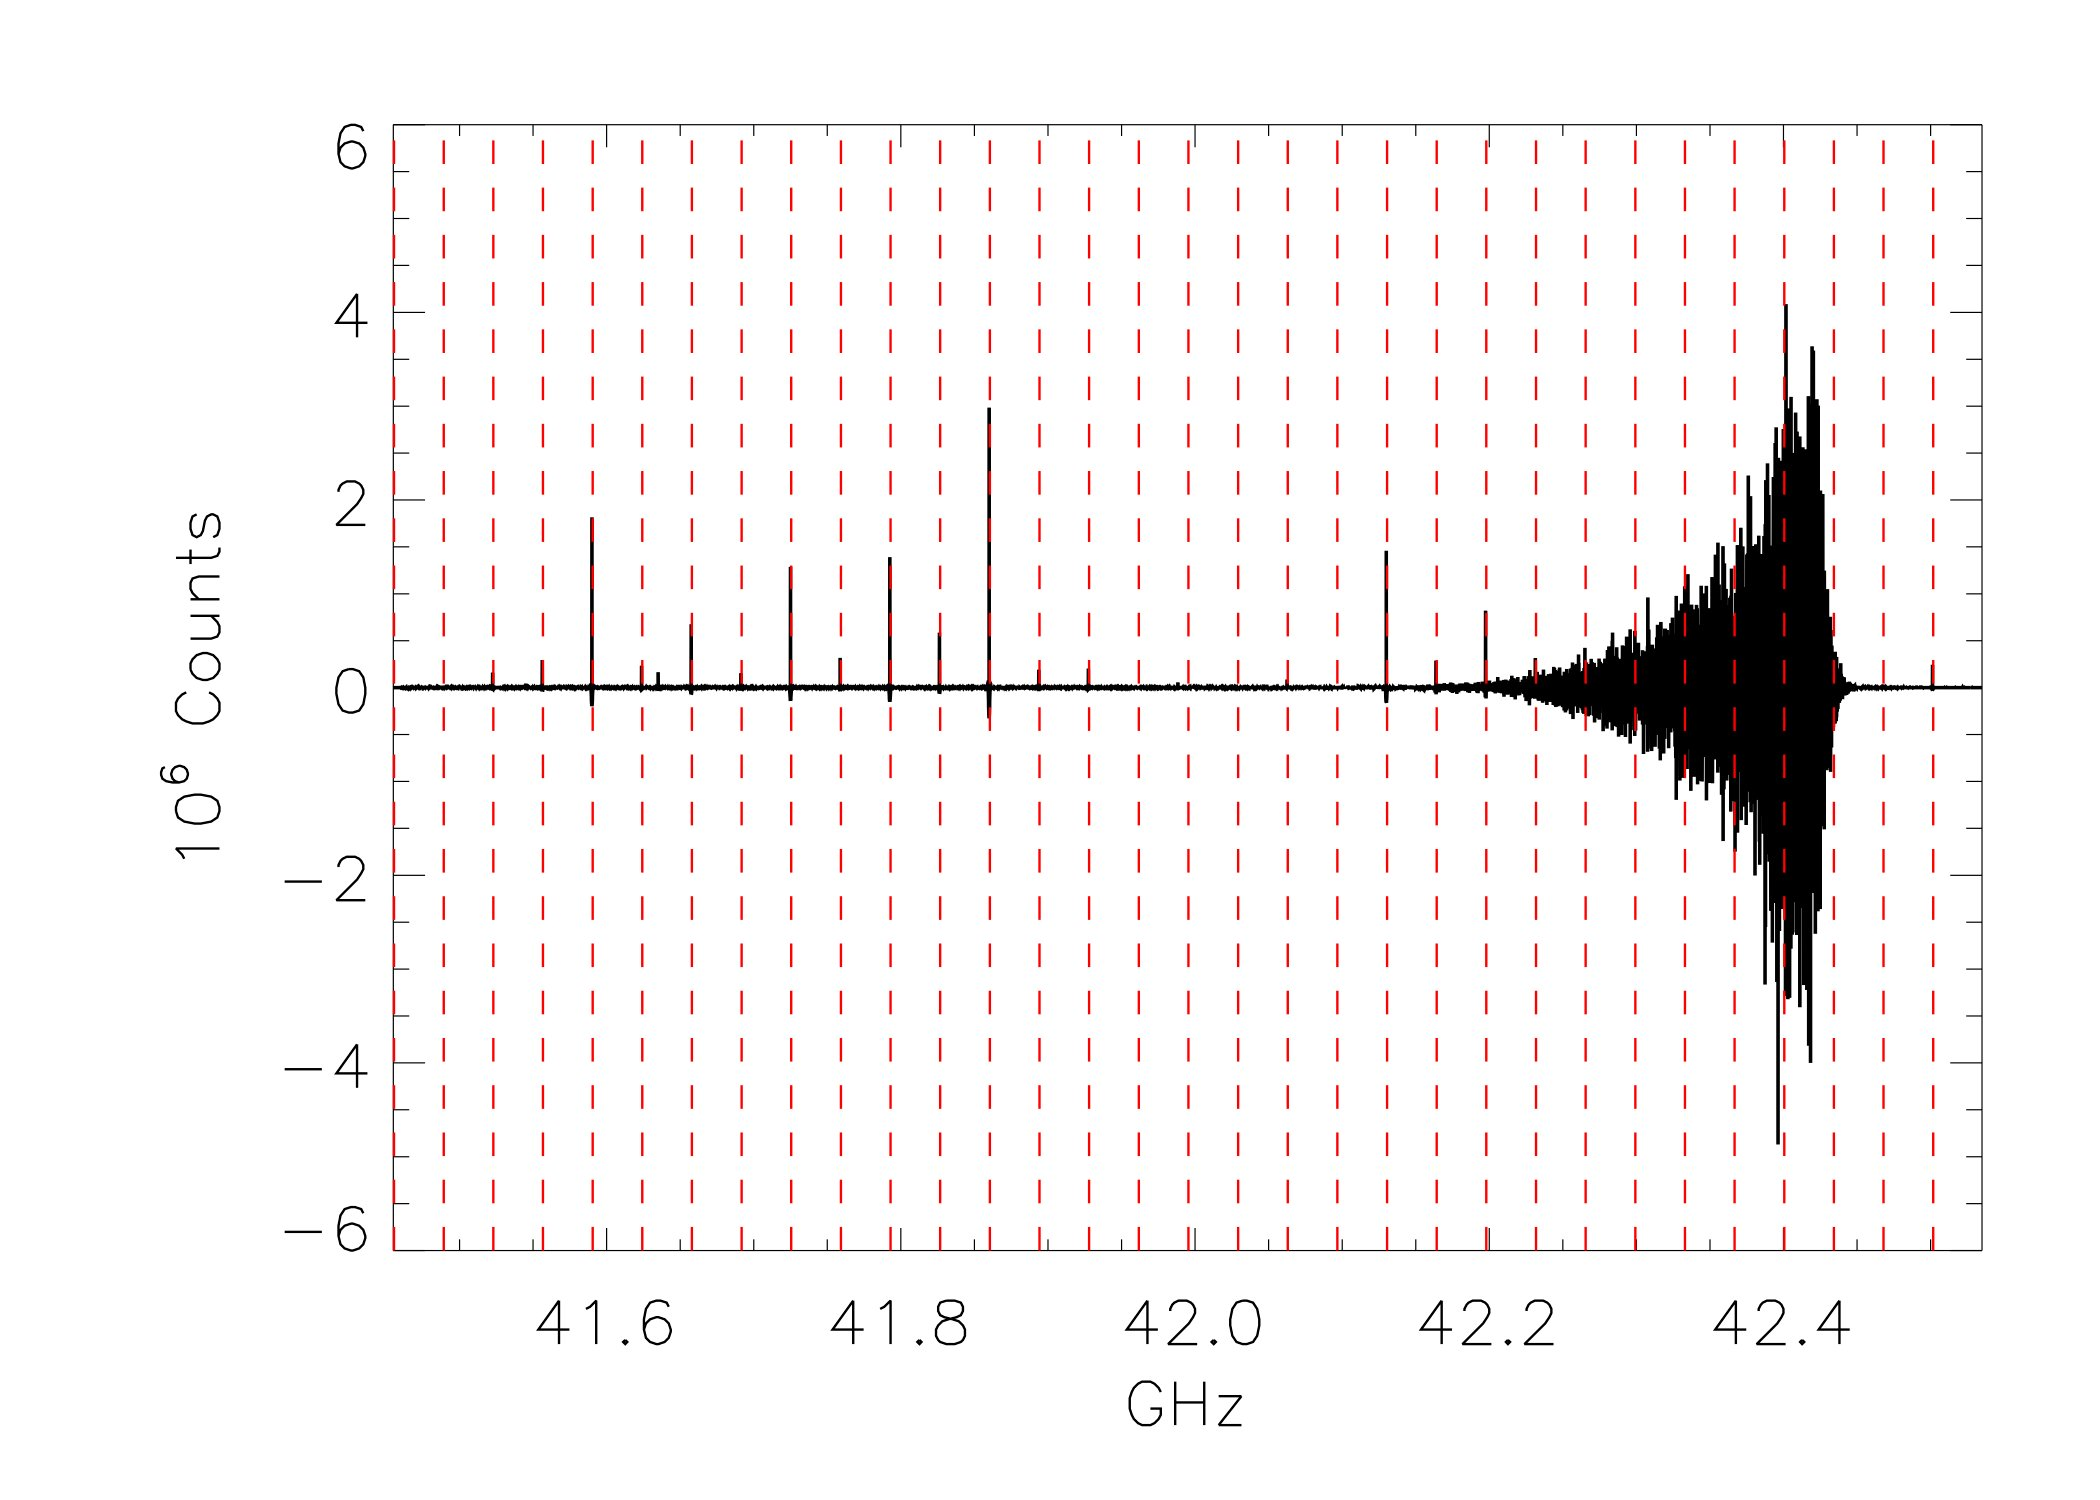
\includegraphics[width=1.\linewidth]{filt_with_spikes.jpg}
\caption[Data from Figure~\ref{fig:vegas_spurs} after the high pass filter]
{Data from Figure~\ref{fig:vegas_spurs} after the high pass filter in 
black, with the vertical red lines denoting the locations of the spurs 
as dictated by Equation~\ref{eq:vegas_spikeeq}}
\label{fig:vegas_spurcalc}
\end{figure}

\noindent It is important to keep in mind that 
$\nu_{\rm s,c}=\mathcal{D}(\nu_{\rm s, r})$; the central sky frequency may be 
shifted by a function $\mathcal{D}$ from the requested sky frequency, 
$\nu_{s, r}$ (e.g. via doppler tracking) . The value of $\nu_{\rm V,c}$ is 
dependent on which mode is used, and is not as straightforward when using 
the low bandwidth (higher resolution) modes 11-29. For modes 4-29, the FFT of 
the raw time series from the ADCs is not performed on the FPGA but on 
external GPUs, which further filter the bandwidth (allowing higher resolution), 
and thus all 33 spurs are not be present in these modes. This filtering in 
the GPU modes also causes $\nu_{\rm V,c}$ to not simply equal to $f_{\rm s}/4$ in 
these cases as it is in modes 1-3. Additionally, for modes 4-29, the signal 
is decimated after being read by the ADCs, and requires an additional scaling 
to be included into Equation~\ref{eq:vegas_spikeeq}.  Table~\ref{tab:vegas_centtbl} 
lists $\nu_{\rm V,c}$ for the various modes. The exact formula for 
these modes is still being worked out, and will be included as soon as 
possible.

\begin{table}[h]
\begin{center}
\caption[$\nu_{\rm V,c}$ for each VEGAS mode]
{$\nu_{\rm V,c}$ for each VEGAS mode}
\label{tab:vegas_centtbl}
\begin{tabular}{| c | c |}
\hline
modes & $\nu_{\rm V,c}$ \\ \hline
1,2&750\\
3&540\\
4-6&750\\
7-9&400\\
10-29&TBD\\
\hline
\end{tabular}
\end{center}
\end{table}

These spurs are relatively stable: $\nu_{\rm spurs}$ will remain constant 
(for a given mode) and the magnitude of the spurs is relatively constant. 
These features are also quite small by most standards (Spurious Free 
Dynamic Range no more than -60dBc), but nevertheless can be problematic 
when looking for faint narrow features. The stability of these features 
allows them to be removed by standard data practices (such as position 
and/or frequency switching), but they are an added noise source which can 
bleed through to the final product. Due to the limited and often 
negligible effect of these spurs, we do not automatically interpolate across 
them, but let the user decide how to handle those channels. A tool for 
locating these spurs within GBTIDL is forthcoming.
